\documentclass[12pt, a4paper]{article}
\usepackage{import}
\usepackage{preamble}

\title{Equivalent Circuits}
\date{\(10^\mathrm{{th}}\) November 2022}
\author{Lee Farrugia}

\begin{document}
    
\maketitle
\thispagestyle{titlepagestyle}
\pagestyle{mystyle}

\section{Abstract}
The project is concerned with the data analysis on provided values for the given values of the reflection coefficient and transmission coefficient of an open-ended coaxial-line probe. This was done in order to obtain values for the complex permittivity of two unknown materials at varying frequencies, which turned out to ultimately be Methanol and 0.1\% Sodium Chloride (NaCl). The values that were calculated were compared to a given data set of complex permittivity for each material. This comparison was conducted in two ways, initially through the visual comparison of the trendline obtained for the two data sets, followed by the direct comparison of four random points from the whole data sets that were calculated and that were given. From the findings, the data for the NaCl should be retaken in order to confirm whether errors occurred when originally taking the readings or whether the data set for the given complex permittivity is incorrect.

\section{Introduction \& Theoretical Background}
The use of open-ended coaxial probes to measure the complex permittivity are used as they are non-invasive and non-destructive to the materials being checked. However, those are not the only advantages this method provides. This method can be utilised to allow for bandwidth measurement and easy sampling \parencite{liao2011accurate}. This method can be used to measure the microwave complex permittivity of dielectric materials including lossy dielectrics. As the relationship between the reflection coefficient and transmission coefficient is quite complex, the equivalent circuit method is used to simplify this relationship \parencite{stuchly1982equivalent}. This is quite useful when dealing with lossy dielectrics and biological tissues, as the biological tissues are not only made up of one type of material but rather of multiple types of tissues in one single sample. Another example of the use of this method is explored in \cite{zajivcek2006evaluation}, where they discuss the relationship of the complex permittivity and the transmission of healthy tissues and tumour tissues. They further discuss how this method could be used to image people using non-ionising radiation.

\section{Materials \& Methods}
\subsection{Language and Packages}
Python 3.10.8, Numpy, Pandas, Matplotlib.pyplot \,.
\subsection{Methodology}
\begin{enumerate}
    \item The data provided for both methanol and sodium chloride was imported into the program and each sheet was given its own \mintinline{py}{pandas} data frame.
    \item The average for the real and imaginary parts at each frequency was calculated for each standard material, i.e. air, short, di-ionised water.
    \item The averages calculated in the previous section were used to calculate the \(\rho\) of each material. These were then used to calculate the \(\Delta\)s found in the equation.
    \item The equation used was:
            \begin{equation}
                \varepsilon_m = -\frac{\Delta_{m2}\Delta_{13}}{\Delta_{m1}\Delta_{32}}\varepsilon_3 - \frac{\Delta_{m3}\Delta_{21}}{\Delta_{m1}\Delta_{32}}\varepsilon_1
            \end{equation}
    \item The average for the real part and imaginary part of the data for the complex permittivity was calculated.
    \item The obtained values for the complex permittivity and the averages of the data given were plotted against each other.
    \item Specific points of the data were printed in order to be compared to each other.
\end{enumerate}

\section{Results \& Discussion}
In~\cite{marsland1987dielectric} the error correction was described as follows:
\begin{itemize}
    \item Calculate \textbf{E}.
    \item Use the calculated \textbf{E} to correct subsequent errors that arise from the measurements.
\end{itemize}
However, as \textbf{E} is not necessary, one can substitute the three known admittance values (of air, short and de-ionised water) along with their respective reflective-coefficient thus, cancelling out the \textbf{E} terms.

As can be seen in~\cite{marsland1987dielectric} the admittance of the probe can be modelled in two ways:
\begin{align}
    y(\omega, \varepsilon_r) &= G_0 Z_0 \varepsilon_r^{\frac{5}{2}} + j \omega Z_0(\varepsilon_r C_0 + C_f) ,  \label{eq: admittance model 1} \\
    y(\omega, \varepsilon_r) &= \omega Z_0(\varepsilon_r C_0 + C_f)\,, \label{eq: admittance model 2}
\end{align}
called the admittance model 1 and admittance model 2 respectively, where \(\omega\) is the angular frequency, \(\varepsilon_r\) is the relative permittivity of the material in which the probe is embedded/immersed in, \(G_0\) is the free-space radiation conductance, \(\varepsilon_r C_0\) is the capacitance which represents the fringing field in the external dielectric material, \(C_f\) is the capacitance which represents the fringing field in the Teflon dielectric of the cable, which usually is \(C_0 \gg C_f\)\,. However, only the admittance model 1 is considered in~\cite{marsland1987dielectric}. Applying a simple linear transformation to the equation~\ref{eq: admittance model 1}, we obtain:
\begin{equation}
    y^{\prime}(\omega, \varepsilon_r) = \left(\frac{1}{j \omega C_0 Z_0}\right)\, \cdot \,y(\omega , \varepsilon_r) - \left(\frac{C_f}{C_0}\right) , \label{eq: admittance model 1 transformed}
\end{equation}
and using equation~\ref{eq: admittance model 1}:
\begin{equation}
    y^{\prime}(\omega, \varepsilon_r) = \varepsilon_r + G_n \varepsilon_r^\frac{5}{2} , \label{eq: admittance model 1 substitution}
\end{equation}
where \(G_n = \frac{G_0}{j\omega C_0}\). This satisfies the linear transformation due to the cross-ratio invariance, which can be further expanded to:
\begin{equation}
    \frac{(\rho_m - \rho_1)(\rho_3 - \rho_1)}{(\rho_m - \rho_2)(\rho_1 - \rho_3)} = \frac{(y^{\prime}_m - y^{\prime}_1)(y^{\prime}_3 - y^{\prime}_2)}{(y^{\prime}_m - y^{\prime}_2)(y^{\prime}_1 - y^{\prime}_2)}\,. \label{eq: opening model 1 subs}
\end{equation}
Expanding equation~\ref{eq: opening model 1 subs} to its \(5^{\text{th}}\) order polynomial, we obtain:
\begin{equation}
    G_n \varepsilon_m^{\frac{5}{2}} + \varepsilon_m + \left[\frac{\Delta_{m1} \Delta_{32} y^{\prime}_3 y^{\prime}_2 + \Delta_{m2} \Delta_{13} y^{\prime}_1 y^{\prime}_3 + \Delta_{m3} \Delta_{21} y^{\prime}_2 y^{\prime}_1}{\Delta_{m1} \Delta{32} y^{\prime}_1 + \Delta_{m2} \Delta{12} y^{\prime}_2 + \Delta_{m3} \Delta{21} y^{\prime}_3}\right] = 0\,. \label{eq: big substitution}
\end{equation}
By applying the short-circuit simplification and setting the termination 1 as a short circuit we obtain:
\begin{equation}
    G_n \varepsilon_m^{\frac{5}{2}} + \varepsilon_m + \left[\frac{\Delta_{m2}\Delta_{13}}{\Delta_{m1}\Delta_{32}} y^{\prime}_3 + \frac{\Delta_{m3}\Delta_{21}}{\Delta_{m1}\Delta_{32}} y^{\prime}_2\right] = 0 \, \label{eq: simplification of big subsitution}
\end{equation}
as \(y^{\prime}_1 \rightarrow \infty\). By omitting the \(G_n\) in equation~\ref{eq: simplification of big subsitution} and in \(y^{\prime}(\omega, \varepsilon_r) = \varepsilon_r + G_n \varepsilon_r^{\frac{5}{2}}\) we obtain:
\begin{equation}
    \varepsilon_m = - \frac{\Delta_{m2}\Delta_{13}}{\Delta_{m1}\Delta_{32}} \varepsilon_3 - \frac{\Delta_{m3}\Delta_{21}}{\Delta_{m1}\Delta_{32}} \varepsilon_2 \,. \label{eq: final equation}
\end{equation}

The complex permittivity of methanol was calculated by first finding the averages of the real and imaginary parts provided in the given data. These averages were then used in order to calculate the \(\rho\) of each material and this was then inputted in equation~\ref{eq: final equation}. One should note that the start of the data points obtained correlate with the averages of the complex permittivity provided in the data given. However, the data points veer off course from the trendline of the given data for the complex permittivity as can be seen in figure~\ref{fig: Methanol Graph}, where the dotted line is the trendline for the given data, while the whole line is the calculated trendline. This can be seen as well in the data in table~\ref{tab: Table 1} where the values start off similar but then vary at higher frequencies. These variations may have arisen due to the errors as mentioned in~\cite{marsland1987dielectric}, i.e.\,the simplification of the admittance model 1. 

\begin{figure}[H]
    \centering
    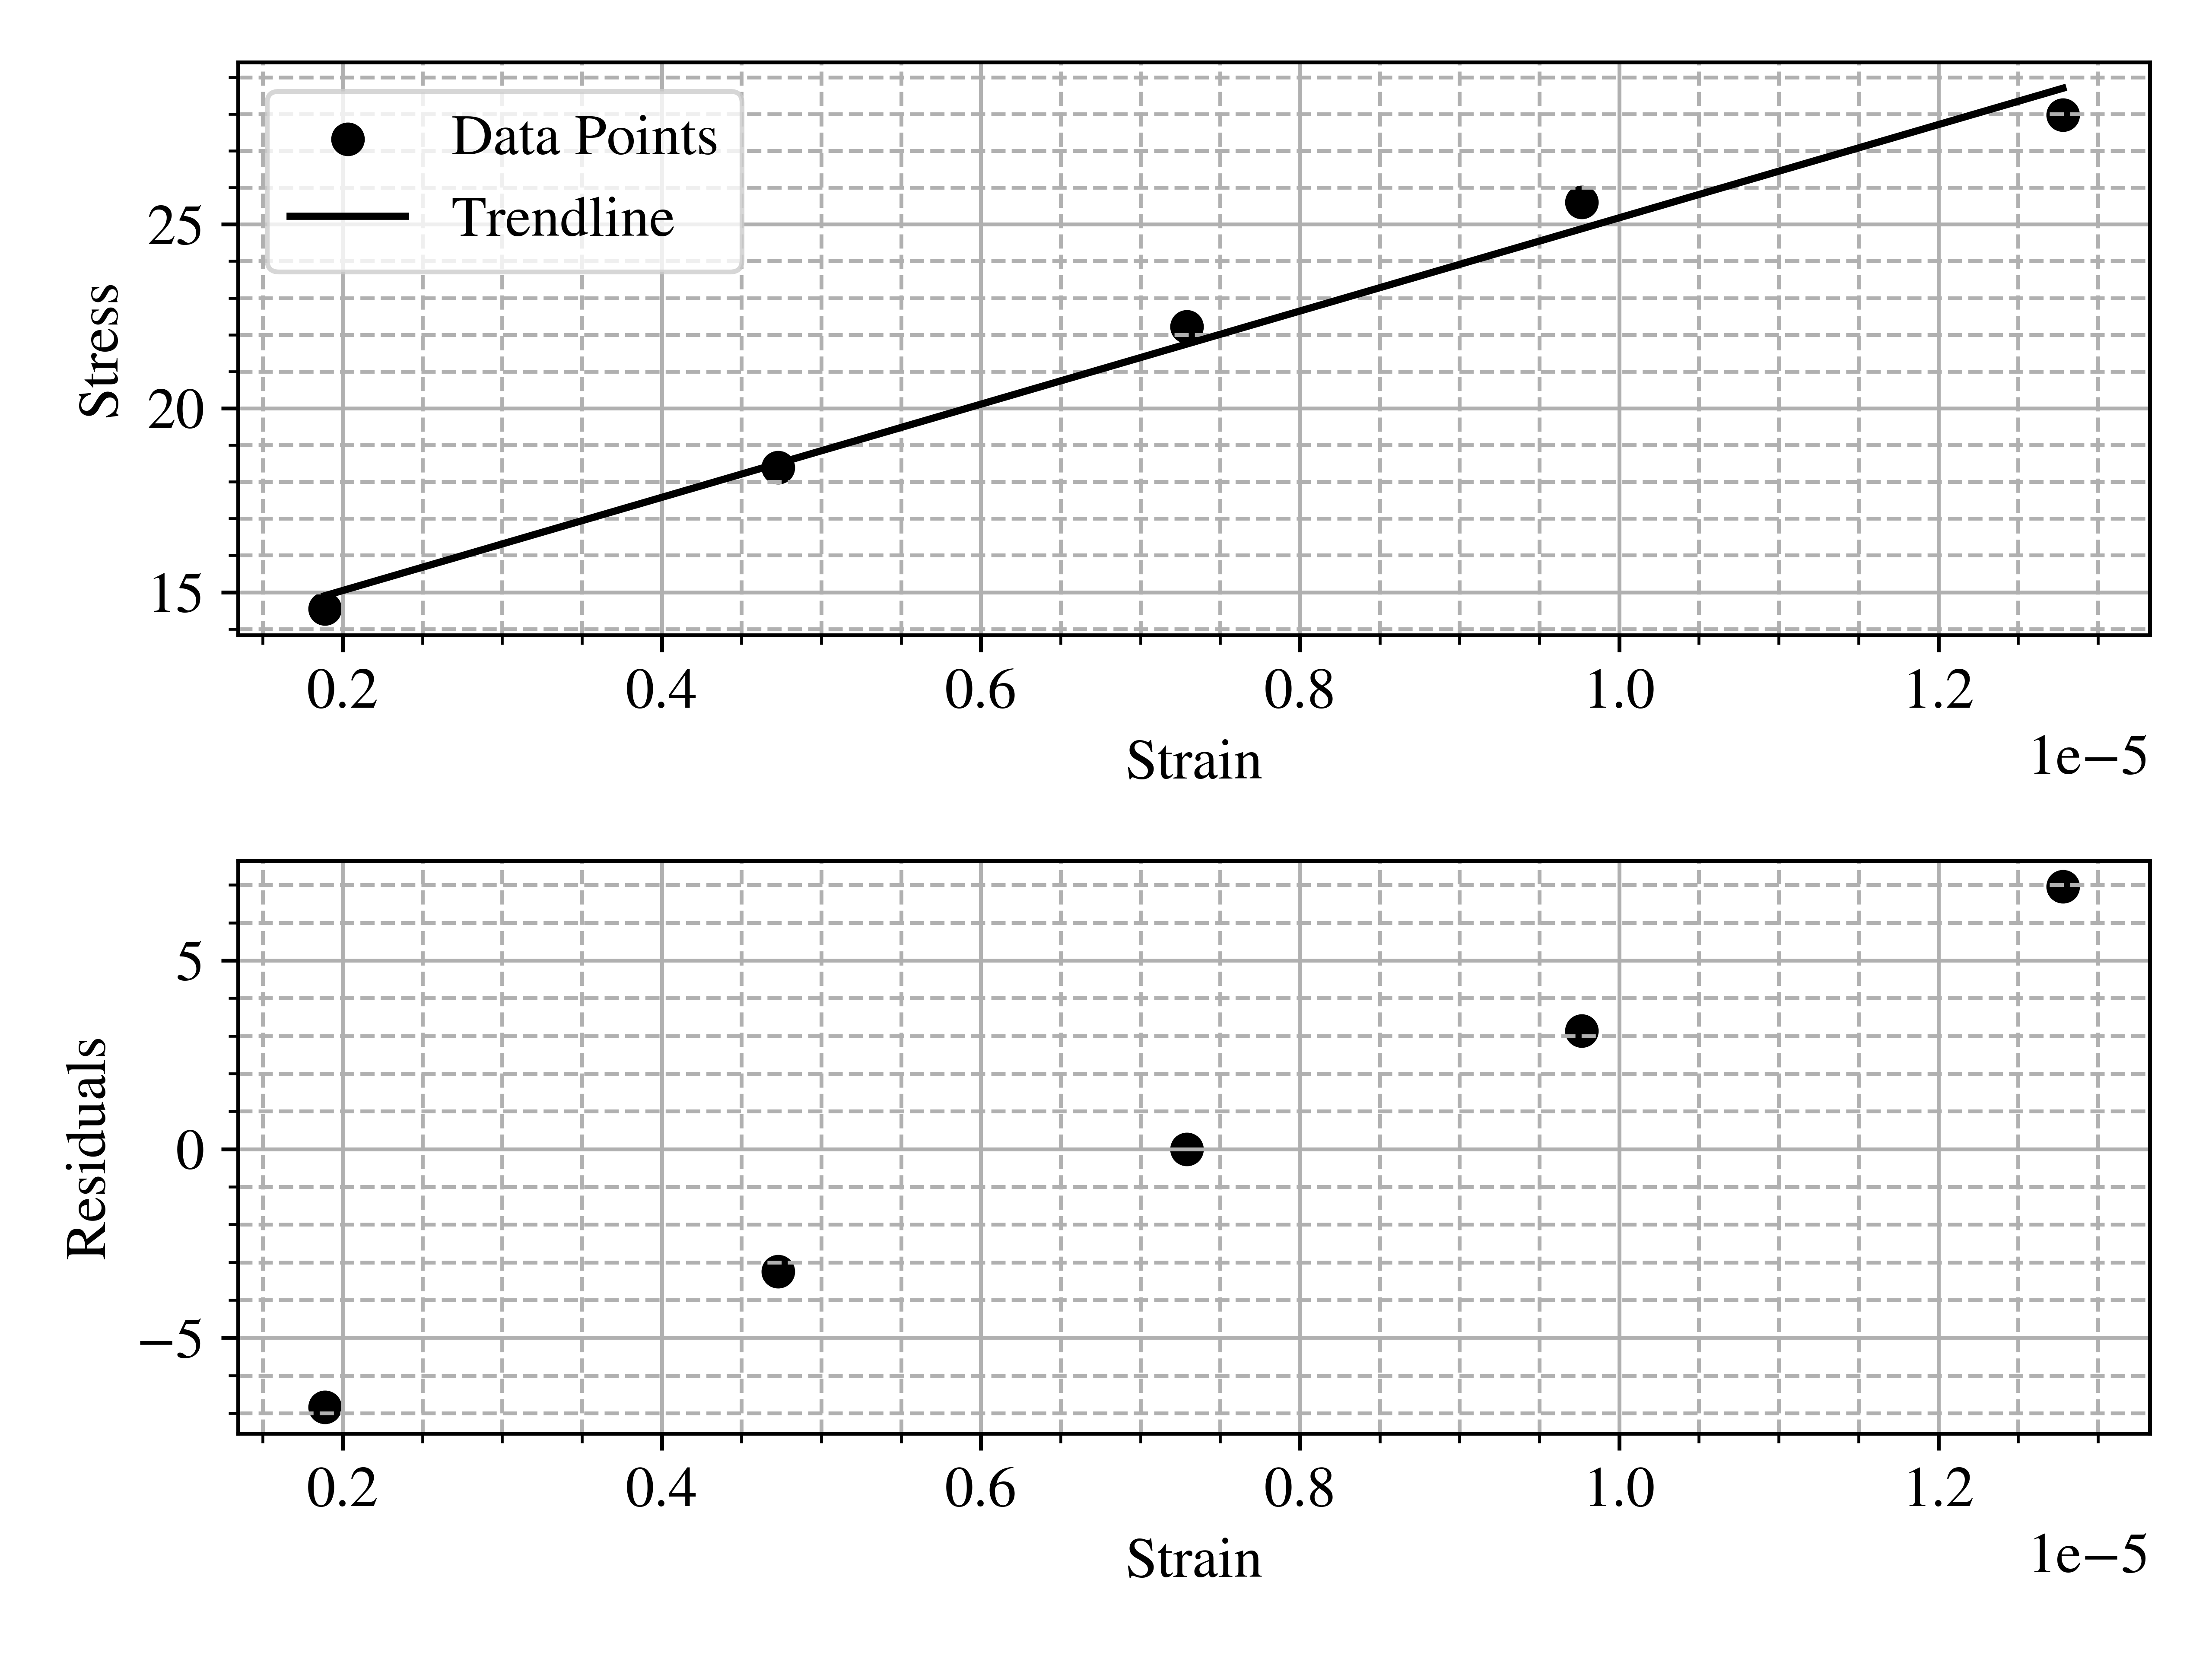
\includegraphics[width = 0.7\textwidth]{Plot1.png}\caption{A graph of the complex permittivity at each frequency for Methanol}\label{fig: Methanol Graph}
\end{figure}

\begin{table}[H]
    \centering
    \begin{tabular}{ccccc}
    \hline
    Frequency/Hz &
      \(\varepsilon_{\mathrm{calculated}}\) &
      \(\varepsilon_{\mathrm{given}}\) \\
      \(\times 10^8\)& & \\ \hline \hline
      5.00   & \(35.15+3.22j\)  & \(35.13-5.07j\)  \\
      40.15  & \(25.31+6.19j\)  & \(17.81-13.83j\) \\
      87.65  & \(20.85+0.76j\)  & \(10.17-8.99j\)  \\
      100.00 & \(11.89+1.19j\)  & \(9.49-8.14j\)   \\
      \hline
    \end{tabular}
    \caption{A table of four different data points for methanol}\label{tab: Table 1}
\end{table}

The complex permittivity of NaCl was found in the same way as the complex permittivity of methanol, but, it can be clearly seen from both the graph and the tabulated results that they do not match the given values of permittivity, figure~\ref{fig: NaCl Graph}, table~\ref{tab: Table 2} respectively. These large variations may not only be the result of the simplification mentioned in~\cite{marsland1987dielectric}, but also the procedure might not have been adhered to correctly. Furthermore, if the setup was not set up as indicated in the diagram as seen in \cite{marsland1987dielectric}, any gaps introduced in the setup will have directly affected the reflection-coefficient, as less of the wave will have been reflected. Furthermore, as \cite{marsland1987dielectric} suggest, the probe must be cleaned between each measurement. These precautions mentioned in~\cite{marsland1987dielectric} would help to reduce the compounding effect of errors in the experiment and would thus help in obtaining a more accurate result. Therefore, it is suggested that the experiment should be repeated with these precautions in mind in order to obtain new data. However, if the precautions obtained by this repetition match what is seen here it would suggest that the given data for the complex permittivity of NaCl would have been the issue and would thus have to be investigated further.

\begin{figure}[H]
    \centering
    \includegraphics[width = 0.7\textwidth]{Plot2.png}\caption{A graph of the complex permittivity at each frequency for Sodium Chloride}\label{fig: NaCl Graph}
\end{figure}

\begin{table}[H]
    \centering
    \begin{tabular}{ccc}
    \hline
    Frequency/Hz &
      \(\varepsilon_{\mathrm{calculated}}\) &
      \(\varepsilon_{\mathrm{given}}\) \\
      \(\times 10^8\)& & \\ \hline \hline
      5.00   & \(82.94+41.57j\) & \(86.41-48.50j\) \\
      40.15  & \(80.60+4.30j\)  & \(82.00-21.69j\) \\
      87.65  & \(80.93+1.69j\)  & \(71.63-32.25j\) \\
      100.00 & \(81.91+2.70j\)  & \(68.40-34.31j\) \\ \hline
    \end{tabular}
    \caption{A table of four different data points for NaCl}\label{tab: Table 2}
\end{table}

\section{Conclusion}
In conclusion, by following the methodology and precautions outlined by~\cite{marsland1987dielectric} one can obtain the complex permittivity of materials. From the data set given, one can conclude that the calculated methanol complex permittivity somewhat resembles the trend of the given complex permittivity although at higher frequencies it does veer away from the given trendline. However, in the case of the calculated complex permittivity of NaCl the trendline is extremely inaccurate when compared to the given complex permittivity which can be the result of compounding errors as discussed above. Thus, the readings for NaCl should be retaken in order to obtain better results.

\section{References}
\printbibliography[heading = none]

\section{Appendix}
\begin{minted}{py}
import numpy as np
import pandas as pd
import matplotlib.pyplot as plt

# importing data to different dataframes for each sheet
data_air = pd.read_excel('Data.xlsx', 0)
data_short = pd.read_excel('Data.xlsx', 1)
data_water = pd.read_excel('Data.xlsx', 2)
data_methanol = pd.read_excel('Data.xlsx', 3).dropna()
data_NaCl = pd.read_excel('Data.xlsx', 4).dropna()
e_methanol = pd.read_excel('Data.xlsx', 5).dropna()
e_NaCl = pd.read_excel('Data.xlsx', 6).dropna()

# defining the frequency variable
frequency = np.array(data_air['%freq[Hz]'])

# finding the average of the real part of air
air_real_avg = data_air[['Real (S11) R1', 'Real (S11) R2', 'Real (S11) R3', 'Real (S11) R4' , 'Real (S11) R5', 'Real (S11) R6']].mean(axis=1)
data_air['Real Avg'] = air_real_avg

# finding the average of the imaginary part of air
air_imaginary_avg = data_air[['Imag (S11) R1', 'Imag (S11) R2', 'Imag (S11) R3', 'Imag (S11) R4' , 'Imag (S11) R5', 'Imag (S11) R6']].mean(axis=1)
data_air['Imag Avg'] = air_imaginary_avg

# finding the average of the real part of water
water_real_avg = data_water[['Real (S11) R1', 'Real (S11) R2', 'Real (S11) R3', 'Real (S11) R4' , 'Real (S11) R5', 'Real (S11) R6']].mean(axis=1)
data_water['Real Avg'] = water_real_avg

# finding the average of the imaginary part of water
water_imaginary_avg = data_water[['Imag (S11) R1', 'Imag (S11) R2', 'Imag (S11) R3', 'Imag (S11) R4' , 'Imag (S11) R5', 'Imag (S11) R6']].mean(axis=1)
data_water['Imag Avg'] = water_imaginary_avg

# finding the average of the real part of methanol
methanol_real_avg = data_methanol[['Real (S11) R1', 'Real (S11) R2', 'Real (S11) R3', 'Real (S11) R4' , 'Real (S11) R5', 'Real (S11) R6']].mean(axis=1)
data_methanol['Real Avg'] = methanol_real_avg

# finding the average of the imaginary part of methanol
methanol_imaginary_avg = data_methanol[['Imag (S11) R1', 'Imag (S11) R2', 'Imag (S11) R3', 'Imag (S11) R4' , 'Imag (S11) R5', 'Imag (S11) R6']].mean(axis=1)
data_methanol['Imag Avg'] = methanol_imaginary_avg

# finding the average of the real part of NaCl
NaCl_real_avg = data_NaCl[['Real (S11) R1', 'Real (S11) R2', 'Real (S11) R3', 'Real (S11) R4' , 'Real (S11) R5', 'Real (S11) R6']].mean(axis=1)
data_NaCl['Real Avg'] = NaCl_real_avg

# finding the average of the imaginary part of NaCl
NaCl_imaginary_avg = data_NaCl[['Imag (S11) R1', 'Imag (S11) R2', 'Imag (S11) R3', 'Imag (S11) R4' , 'Imag (S11) R5', 'Imag (S11) R6']].mean(axis=1)
data_NaCl['Imag Avg'] = NaCl_imaginary_avg

# finding the average of the given real permittivity of methanol
e_methanol_real_avg = e_methanol[["e'_R1","e'_R2","e'_R3"]].mean(axis=1)
e_methanol['Real Avg'] = e_methanol_real_avg

# finding the average of the given imaginary permittivity of methanol
e_methanol_imaginary_avg = e_methanol[["e''_R1","e''_R2","e''_R3"]].mean(axis=1)
e_methanol['Imag Avg'] = e_methanol_imaginary_avg

# finding the average of the given real permittivity of NaCl
e_NaCl_real_avg = e_NaCl[["e'_R1","e'_R2","e'_R3"]].mean(axis=1)
e_NaCl['Real Avg'] = e_NaCl_real_avg

# finding the average of the given imaginary permittivity of NaCl
e_NaCl_imaginary_avg = e_NaCl[["e''_R1","e''_R2","e''_R3"]].mean(axis=1)
e_NaCl['Imag Avg'] = e_NaCl_imaginary_avg

# defining the different perimittivity as numpy array
short_r_avg = data_short['re:Trc1_S11'].to_numpy()
short_i_avg = data_short['im:Trc1_S11'].to_numpy()

air_r_avg = data_air['Real Avg'].to_numpy()
air_i_avg = data_air['Imag Avg'].to_numpy()

water_r_avg = data_water['Real Avg'].to_numpy()
water_i_avg = data_water['Imag Avg'].to_numpy()

methanol_r_avg = data_methanol['Real Avg'].to_numpy()
methanol_i_avg = data_methanol['Imag Avg'].to_numpy()

NaCl_r_avg = data_NaCl['Real Avg'].to_numpy()
NaCl_i_avg = data_NaCl['Imag Avg'].to_numpy()

e_methanol_r_avg = e_methanol['Real Avg'].to_numpy()
e_methanol_i_avg = e_methanol['Imag Avg'].to_numpy()

e_NaCl_r_avg = e_NaCl['Real Avg'].to_numpy()
e_NaCl_i_avg = e_NaCl['Imag Avg'].to_numpy()

# creating the complex numbers from the averages
air_complex = air_r_avg - (1j * air_i_avg)
short_complex = short_r_avg - (1j * short_i_avg)
water_complex = water_r_avg - (1j * water_i_avg)
methanol_complex = methanol_r_avg - (1j * methanol_i_avg)
NaCl_complex = NaCl_r_avg - (1j * NaCl_i_avg)
e_methanol_c = e_methanol_r_avg - (1j * e_methanol_i_avg)
e_NaCl_c = e_NaCl_r_avg - (1j * e_NaCl_i_avg)

# calculating the different deltas required in the equation
delta_13 = np.subtract(short_complex, water_complex)
delta_21 = np.subtract(air_complex, short_complex)
delta_23 = np.subtract(air_complex, water_complex)
delta_32 = np.subtract(water_complex, air_complex)
delta_m1_methanol = np.subtract(methanol_complex, short_complex)
delta_m2_methanol = np.subtract(methanol_complex, air_complex)
delta_m3_methanol = np.subtract(methanol_complex, water_complex)
delta_m1_NaCl = np.subtract(NaCl_complex, short_complex)
delta_m2_NaCl = np.subtract(NaCl_complex, air_complex)
delta_m3_NaCl = np.subtract(NaCl_complex, water_complex)

# using the equation and values to calculate the complex permittivity
e_methanol = -1 * (((delta_m2_methanol * delta_13) / (delta_m1_methanol * delta_32)) * 80.5) - (((delta_m3_methanol * delta_21) / (delta_m1_methanol * delta_32)) * 1)
e_NaCl = -1 * (((delta_m2_NaCl * delta_13) / (delta_m1_NaCl * delta_32)) * 80.5) - (((delta_m3_NaCl * delta_21) / (delta_m1_NaCl * delta_32)) * 1)

# taking the real parts only
methanol_real = np.real(e_methanol)
e_methanol_real = np.real(e_methanol_c)
NaCl_real = np.real(e_NaCl)
e_NaCl_real = np.real(e_NaCl_c)

# polyfit calculated methanol
coefficients, cov = np.polyfit(frequency, methanol_real, 5, cov=True)
poly_function = np.poly1d(coefficients)
trendline_c_m = poly_function(frequency)

# polyfit given methanol
coefficients, cov = np.polyfit(frequency, e_methanol_real, 5, cov=True)
poly_function = np.poly1d(coefficients)
trendline_g_m = poly_function(frequency)

# polyfit calculated NaCl
coefficients, cov = np.polyfit(frequency, NaCl_real, 5, cov=True)
poly_function = np.poly1d(coefficients)
trendline_c_n = poly_function(frequency)

# polyfit given NaCl
coefficients, cov = np.polyfit(frequency, e_NaCl_real, 5, cov=True)
poly_function = np.poly1d(coefficients)
trendline_g_n = poly_function(frequency)

# value comparisons
positions = (0, 74, 174, 200)
for i in positions:
    print(f'The calculated permittivity at data point {i+1} for methanol is:{e_methanol[i]:.2f}, while the given value is: {e_methanol_c[i]:.2f}')
    print(f'The calculated permittivity at data point {i+1} for NaCl is:{e_NaCl[i]:.2f}, while the given value is: {e_NaCl_c[i]:.2f}')

# plotting the data for methanol
plt.figure(figsize=(7.5, 10.5))
plt.rcParams['font.family'] = 'STIXGeneral'
plt.rcParams['mathtext.fontset'] = 'stix'
plt.rcParams['font.size'] = 12
plt.rcParams['font.weight'] = 'normal'
plt.minorticks_on()
plt.grid(visible=True, which='major', linestyle='-')
plt.grid(visible=True, which='minor', linestyle='--')

plt.scatter(frequency, methanol_real, color='k', label='Calculated')
plt.plot(frequency, trendline_c_m, color = 'k', label='Calculated')
plt.scatter(frequency, e_methanol_real, color='grey', label='Given')
plt.plot(frequency, trendline_g_m, '--',  color = 'k', label = 'Given')
plt.xlabel('f/Hz')
plt.ylabel(r'$\mathrm{\epsilon_{methanol}}$')
plt.title('Complex Permittivity of Methanol vs Frequency')
plt.legend()
plt.savefig('Plot1.pdf', dpi=800)
plt.show()
plt.close()

# plotting the data of NaCl
plt.figure(figsize=(7.5, 10.5))
plt.rcParams['font.family'] = 'STIXGeneral'
plt.rcParams['mathtext.fontset'] = 'stix'
plt.rcParams['font.size'] = 12
plt.rcParams['font.weight'] = 'normal'
plt.minorticks_on()
plt.grid(visible=True, which='major', linestyle='-')
plt.grid(visible=True, which='minor', linestyle='--')

plt.scatter(frequency, NaCl_real, color='k', label='Calculated')
plt.plot(frequency, trendline_c_n, color = 'k', label='Calculated')
plt.scatter(frequency, e_NaCl_real, color='grey', label='Given')
plt.plot(frequency, trendline_g_n, '--',  color = 'k', label = 'Given')
plt.xlabel('f/Hz')
plt.ylabel(r'$\mathrm{\epsilon_{NaCl}}$')
plt.title('Complex Permittivity of NaCl vs Frequency')
plt.legend()
plt.savefig('Plot2.pdf', dpi=800)
plt.show()

\end{minted}

\end{document}